\subsection{Exploratory Data Analysis}
\nestindent

We conduct exploratory analysis on two baselines to identify failure modes that binary correctness reward cannot address.

\subsubsection{Baselines}
\nestindent

\textbf{SFT baseline.}
The Part~2 best SFT checkpoint (\texttt{a4p2-sft-metamath-swiglu}, step 24633), which achieves 15.39\% strict accuracy and 88.93\% parseable rate on GSM8K.
This is the starting point for all RL runs.

\textbf{RL baseline.}
The result of running Karpathy's original RL training script with binary correctness reward only on the SFT checkpoint (467 steps, REINFORCE, no KL regularization).
This is the ``Baseline'' run in our ablation study, achieving \pFourBaselinePassOne\% Pass@1.

\nestunindent
\subsubsection{Baseline Analysis}
\nestindent

\textbf{Response quality.}
We evaluate the RL baseline on 1319 GSM8K test problems, generating 8 samples per problem (Table~\ref{tab:p4-eda-quality}).

\vspace{1em}
\noindent\begin{minipage}{\linewidth}
\centering
\begin{tabular*}{\linewidth}{@{\extracolsep{\fill}}lr}
\toprule
\textbf{Metric} & \textbf{Value} \\
\midrule
Pass@1              & 9.7\%  \\
Pass@8              & 24.9\% \\
Pass@8--Pass@1 gap  & 15.2\% \\
Extraction failure  & 60.3\% \\
Degenerate text     & 32.8\% \\
Near-miss           & 8.5\%  \\
Consistency         & 0.21   \\
Avg.\ response length & 283 tokens \\
Answer magnitude    & median 42, max 2.88M \\
\bottomrule
\end{tabular*}
\addtocounter{table}{1}
\label{tab:p4-eda-quality}
\end{minipage}
\vspace{1em}

The majority of responses are unusable: 60.3\% lack a parseable answer (blocking all gradient signal), 32.8\% degenerate into gibberish (a consequence of no KL regularization), and even among the 8 samples per problem, consistency is only 0.21.
The wide Pass@8--Pass@1 gap (15.2\%) indicates the model can solve many problems but not reliably, suggesting that reward signals which stabilize output quality could improve accuracy without requiring new reasoning capability.
The answer magnitude range (median 42, max 2.88M) means any proximity-based reward must normalize for scale.

RL evaluation uses temperature=1.0 (required for REINFORCE), unlike Part~2's greedy evaluation, so the two accuracy numbers are not directly comparable.
The parseability drop from 88.93\% to 39.7\% likely reflects both stochastic sampling and the absence of KL regularization.

\textbf{Failure mode distribution.}
We classify each of the baseline's 990 failed problems into six categories using a rule-based taxonomy (Table~\ref{tab:taxonomy}).

\vspace{1em}
\noindent\begin{minipage}{\linewidth}
\centering
\begin{tabular*}{\linewidth}{@{\extracolsep{\fill}}l p{0.7\linewidth}}
\toprule
\textbf{Category} & \textbf{Rule} \\
\midrule
Gibberish       & CamelCase token fraction ${>}\,25\%$ or mega-token fraction ${>}\,20\%$ or response length ${<}\,20$ characters. Matches Reward~C's anti-gibberish signals. \\
No answer       & No \texttt{\#\#\#\# <number>} marker and no extractable numbers in the response. \\
Format only     & Contains numbers but not in the expected \texttt{\#\#\#\# <number>} format. \\
No reasoning    & Has \texttt{\#\#\#\#} marker but fewer than 2 non-answer lines and no calculator usage---the model jumped directly to an answer. \\
Arithmetic error & Answer is close to gold (relative error $< 0.5$), with reasoning or calculator usage present. \\
Large error     & Answer is far from gold (relative error $\geq 0.5$), indicating incorrect operations or problem misinterpretation. \\
\bottomrule
\end{tabular*}
\captionof{table}{Rule-based mistake taxonomy. Categories are applied in order; the first matching rule determines the classification.}
\label{tab:taxonomy}
\end{minipage}
\vspace{1em}

\vspace{1em}
\noindent\begin{minipage}{\linewidth}
\centering
\begin{tabular*}{\linewidth}{@{\extracolsep{\fill}}lrr}
\toprule
\textbf{Category} & \textbf{Count} & \textbf{\%} \\
\midrule
No answer        & 273 & 27.6 \\
Format only      & 389 & 39.3 \\
Arithmetic error & 110 & 11.1 \\
Large error      & 186 & 18.8 \\
Gibberish        &  32 &  3.2 \\
\midrule
Total            & 990 &      \\
\bottomrule
\end{tabular*}
\captionof{table}{Baseline error distribution across 990 failed problems (all 8 samples incorrect).}
\label{tab:p4-eda-errors}
\end{minipage}
\vspace{1em}

Format-related failures (no answer + format only) account for 66.9\% of errors, meaning the primary bottleneck is producing parseable output, not reasoning.
Gibberish (3.2\%) captures degenerate token patterns detectable by CamelCase and mega-token heuristics.
A reward that targets format compliance could convert format failures into scoreable responses, while the remaining 29.9\% reasoning errors (arithmetic + large error) require different signals.

\textbf{Reward hacking.}
We examine whether the baseline's ``correct'' responses actually solve the given problem (Figure~\ref{fig:p4-alignment}).

\vspace{1em}
\noindent\begin{minipage}{\linewidth}
\centering
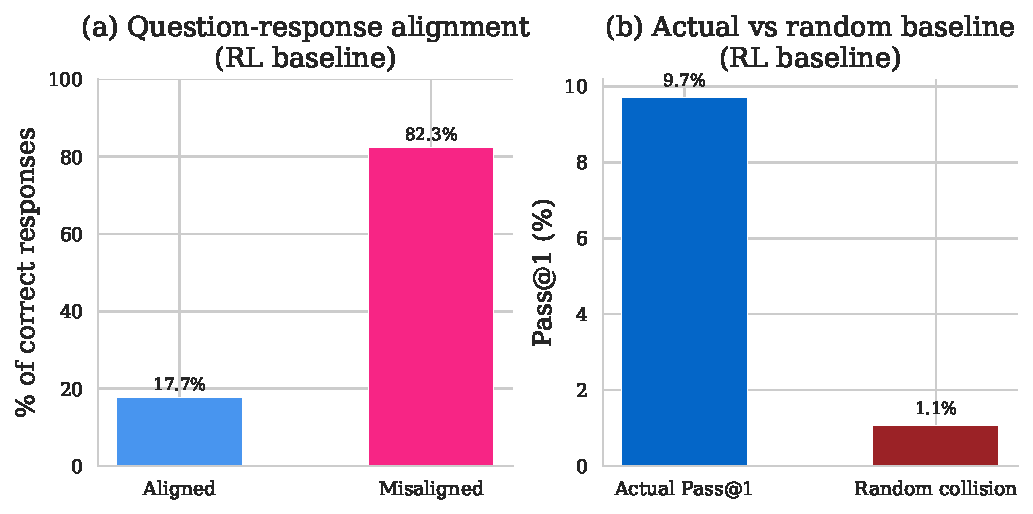
\includegraphics[width=\linewidth]{component/figures/p4/fig_alignment.pdf}
\captionof{figure}{Reward hacking evidence. (a)~Fraction of correct responses sharing proper nouns with the question ($\sim$18\%). (b)~Actual Pass@1 vs.\ random number-collision rate.}
\label{fig:p4-alignment}
\end{minipage}
\vspace{1em}

Only 18\% of ``correct'' responses share proper nouns with the question, suggesting the model rarely engages with the specific problem posed.
Yet the model achieves 9.7\% Pass@1 versus a 1.1\% random number-collision baseline, so it is not purely guessing---it exhibits some crude mathematical competence that lands on plausible answers far more often than chance.
These two findings together paint a picture of a model that can perform generic arithmetic but does so untethered from the input: it produces numerically reasonable outputs without reading the problem, and the binary correctness reward---which checks only the final number---provides no incentive to do otherwise.
This suggests that a reward signal grounding the response in the input (e.g., checking whether entities or quantities from the question appear in the reasoning) could push the model from superficial number-matching toward faithful problem-solving.

\nestunindent
\subsubsection{Key Findings}
\nestindent

The analysis reveals five failure modes that binary correctness reward cannot distinguish or address:
\begin{enumerate}[nosep]
    \item \textbf{Unparseable output} (60.3\%): responses without a \texttt{\#\#\#\# <number>} marker receive zero reward, blocking all gradient signal.
    \item \textbf{Wrong but close answers} (8.5\% near-miss): responses off by 1 receive the same zero reward as those off by 10{,}000.
    \item \textbf{Text degeneration} (32.8\% gibberish): without KL regularization, RL training drives responses toward degenerate token patterns.
    \item \textbf{Input-unfaithful reasoning}: only 18\% of ``correct'' responses share proper nouns with the question; the model exhibits crude mathematical competence (9.7\% Pass@1 vs.\ 1.1\% random collision) but largely untethered from the specific problem posed.
    \item \textbf{Indiscriminate zero reward}: format failures, reasoning failures, and near-misses all receive identical zero signal.
\end{enumerate}
These findings motivate the five auxiliary rewards described in Section~\ref{sec:reward-design}: format compliance (1), numeric proximity (2), surface non-degeneracy (3), entity grounding (4), and number grounding (4).

\nestunindent
\nestunindent
